\documentclass[conference]{IEEEtran}
\IEEEoverridecommandlockouts
% The preceding line is only needed to identify funding in the first footnote. If that is unneeded, please comment it out.
\usepackage{cite}
\usepackage{amsmath,amssymb,amsfonts}
\usepackage{algorithmic}
\usepackage{graphicx}
\usepackage{textcomp}
\usepackage{xcolor}
\def\BibTeX{{\rm B\kern-.05em{\sc i\kern-.025em b}\kern-.08em
    T\kern-.1667em\lower.7ex\hbox{E}\kern-.125emX}}

\newcommand{\taskprefix}{CH}
\newcommand{\tasksize}{\normalsize}
\newenvironment{taskenv}[1]{\begin{list}{{\tasksize\sc \theenumi.}}{\usecounter{enumi}
      \settowidth{\labelwidth}{{\tasksize\sc \taskprefix#1-99}}
      \setlength{\leftmargin}{\labelwidth}
      %\addtolength{\leftmargin}{2.0\labelsep}
}}{\end{list}}
\newcounter{task}
\setcounter{task}{-1}
\newcommand{\btask}{\begin{taskenv}{\taskprefix}\setcounter{enumi}{\value{task}}\renewcommand{\theenumi}{\taskprefix$_{\arabic{enumi}}$}}
\newcommand{\etask}{\setcounter{task}{\value{enumi}}\renewcommand{\theenumi}{\arabic{enumi}.}\end{taskenv}}

\begin{document}

\title{Large-scale peer-to-peer network for mobile platforms: Challenges and Experiences\\
%\thanks{DAIS-ITA}
}

\author{\IEEEauthorblockN{Nirmit Desai, Wendy Chong, Heather Achilles, Shahrokh Daijavad}
\IEEEauthorblockA{\textit{IBM T. J. Watson Research Center} \\
%\textit{}\\
Yorktown Heights, NY, USA \\
\{nirmit.desai, wendych, hachilles, shahrokh\}@us.ibm.com}
\and
%\IEEEauthorblockN{Wendy Chong}
%\IEEEauthorblockA{\textit{IBM T. J. Watson Research Center} \\
%\textit{name of organization (of Aff.)}\\
%Yorktown Heights, NY, USA \\
%wendych@us.ibm.com}
%\and
%\IEEEauthorblockN{Heather Achilles}
%\IEEEauthorblockA{\textit{IBM T. J. Watson Research Center} \\
%\textit{name of organization (of Af}\\
%Yorktown Heights, NY, USA \\
%hachilles@us.ibm.com}
%\and
%\IEEEauthorblockN{Shahrokh Daijavad}
%\IEEEauthorblockA{\textit{IBM T. J. Watson Research Center} \\
%\textit{Penn}\\
%Yorktown Heights, NY, USA \\
%shahrokh@us.ibm.com}
\and
\IEEEauthorblockN{Thomas La Porta}
\IEEEauthorblockA{\textit{Dept. of Computer Science and Engineering} \\
\textit{Penn State University}\\
University Park, PA, USA \\
tlp@cse.psu.edu}
%\and
%\IEEEauthorblockN{5\textsuperscript{th} Given Name Surname}
%\IEEEauthorblockA{\textit{dept. name of organization (of Aff.)} \\
%\textit{name of organization (of Aff.)}\\
%City, Country \\
%email address}
%\and
%\IEEEauthorblockN{6\textsuperscript{th} Given Name Surname}
%\IEEEauthorblockA{\textit{dept. name of organization (of Aff.)} \\
%\textit{name of organization (of Aff.)}\\
%City, Country \\
%email address}
}

\maketitle

\begin{abstract}
Peer-to-peer (p2p) networks and Mobile ad hoc networks (MANET) have
been widely studied. However, a real-world deployment for the masses
has remained elusive. Ever-increasing density of mobile devices,
especially in urban areas, has given rise to new applications of p2p
communication. However, the modern smartphone platforms have limited
support for such communications. Further, the issues of battery life,
range, and security remain unaddressed. A key question then is, what
kinds of applications can the modern mobile platforms support and what
challenges remain? This paper identifies a class of applications and
presents a novel p2p architecture called Mesh Network Alerts (MNA) to
support them.  We describe our experiences in deploying MNA as a
real-world peer-to-peer network to millions of users for relaying
severe weather information along with the challenges faced, and the
approaches for addressing them.
\end{abstract}

\begin{IEEEkeywords}
peer-to-peer systems, mobile ad hoc network, delay-tolerant network
\end{IEEEkeywords}

\section{Introduction}
Mobile devices with programmable platforms such as android and iOS
have steadily grown over the last decade, surpassing the 2 billion
mark \footnote{https://www.statista.com/statistics/330695/number-of-smartphone-users-worldwide/}. MANETs
have been greatly studied given their decentralized nature and
potential for new applications
\cite{loo-manet-2011,perkins-ad-hoc-2001}. Most of the prior work on
p2p networks has focused on valuable analytical and simulation-based
study of MANET behavior
\cite{zhang-topology-manet-2015,marti-misbehavior-manet-2000,mauve-pos-routing-manet-2001}. Given
the outstanding practical challenges of physical nodes, real-world
implementations have been limited and have not reached mass scale
\cite{kiess-manet-impl-2007}. However, with the growth of smartphones,
large-scale real-world implementations may become feasible. This paper
describes a real-world implementation of a p2p delay-tolerant network,
called Mesh Network Alerts (MNA), for relaying severe weather
information to millions of mobile device users as part of the Weather
Channel app\footnote{https://weather.com/apps/ibm/meshnetworkalerts}
on both android and iOS platforms.

Before describing MNA, it is critical to identify applications that
need p2p communication, given pervasive Internet connectivity. Doing
so enables us to define key characteristics of such applications and
focus on the challenges in meeting them.  This paper focuses on two
separate classes of applications: communication in
(a) disaster-affected or remote areas and (b) congested networks in
densely populated areas, e.g., sports arenas.  The following are the
key characteristics in these scenarios:

%
\btask
%
\item\label{c:0} No secondary communication infrastructure such as WiFi
  access points to fall back on
\item\label{c:1} Network nodes are mobile, pattern of mobility is not
  predictable
\item\label{c:2} New information may arrive at any time
\item\label{c:3} Trustworthy information is scarce, misinformation and
  rumours are common place
\item\label{c:4}  Small payloads suffice in many cases and information
  stays relevant for a few minutes
\item\label{c:5}  Device battery is a scarce resource, power supply
  for recharging may not be available
\item\label{c:6}  Devices are owned by citizens, deployment of
  special-purpose devices is cost prohibitive
%
\etask
%

The above needs are well-recognized in the industry with several
ambitious attempts to address them, e.g., Google Loon
project\footnote{https://loon.co} and Facebook
Aquilla\footnote{https://en.wikipedia.org/wiki/Facebook\_Aquila},
though with limited impact. Leveraging user mobile devices as peer
nodes for a large-scale deployment has been another theme in the prior
works, e.g., the Serval project
\cite{gardner-stephen-serval-2011}. Serval mesh enables p2p
communication over on-device WiFi radio, but requires root access to
the device via jailbreaking. Although significant leassons have been
learned through these attempts, a mass-scale p2p network for such
applications remains elusive.

A vast majority of the literature has focused on a traditional model
of stateful and reliable networking. Specifically, the nodes maintain
connectivity with peers, routing is optimized with techniques based on
link state or distance vectors
\cite{clausen-olsr-2003,perkins-aodv-2003} focusing on optimizing the
network utilization. Given the application characteristics above, this
paper identifies main practical challenges associated with modern
device platforms and finds novel ways to overcome them.  This leads to
MNA --- a new paradigm in p2p networking that employs connection-less,
delay-tolerant, and zero-routing overhead protocols.  MNA is
implemented on both Android and iOS as an SDK and integrated with the
Weather Channel mobile apps. With extensive experiments and experience
of deploying to almost $10$ million users, MNA represents a way
forward for large-scale p2p networks.

In summary, this paper makes the following key contributions:
\begin{itemize}
\item Identification of a class of applications for p2p and their key
  characteristics
\item A deeper investigation of the practical challenges in supporting
  the above class of applications
\item A novel p2p networking SDK using multiple radio
  channels for modern mobile platforms (Android and iOS)
\item Experimental evaluation and deployment statistics
\end{itemize}

In the following, Section~\ref{sec:challenges} describes the practical
challenges. Section~\ref{sec:architecture} outlines the architectural
details of MNA along with platform-specific implementation issues for
Android and iOS in addressing the challenges. Experimental evaluation
and deployment statistics are presented in Section~\ref{sec:eval}.  A
deeper look at the literature and contrast to MNA is summarized in
Section~\ref{sec:related} with conclusions in
Section~\ref{sec:conclude}.
%
\section{Practical Challenges}
\label{sec:challenges}
%
We present the main challenges for modern mobile device platforms in
meeting the classes of applications described above. These have been
uncovered via extensive experiments and in some cases include direct
feedback from the makers of Android and iOS.
%
\subsection{Operating system constraints}
\label{ch:os}
%
Due to \ref{c:2}, even when a user is not interacting with the weather
app, or worse yet, when the device is not being used at all, the
devices must discover peer devices to receive and formward potentially
life-saving weather information. Although modern mobile operating
systems such as Android and iOS offer APIs to discover and advertise
information to peer devices over WiFi and Bluetooth interfaces,
peer-to-peer connections do not work when the same APIs are accessed
while the app is in the background. Prior works, widely document these
challenges and take the approach of having special access on the
devices, e.g., jail-breaking or rooting
\cite{gardner-stephen-serval-2011}. Clearly, such an approach does not
scale to mass adoption.
%
\subsection{Power constraints}
\label{ch:power}
%
Since devices may be offline when new weather information arrives, MNA
processes on each peer must remain active at all times to be able to
discover new information as soon as it arrives. Further, as there is
no back up infrastructure (\ref{c:0}) and a set of peers in range can
change at any time (\ref{c:1}), each peer is responsible for
constantly forwarding available information to other peers via
advertisements. However, due to \ref{c:5}, the MNA activity must keep
the device battery consumption to a minimum. This is a challenge
because advertising and discovery are power-hungry operations over the
radio channels.
%
\subsection{Testing p2p networks}
%
Given the heterogeneity of devices and operating system distributions
owned by users (\ref{c:6}), it is challenging to test whether or not
MNA functions as expected on a single device. Further, running test
scenarios on a p2p network at large-scale is non-trivial given that a
large number of devices need to take specific coordinated action
followed by coordinated observations to determine whether a test
passes or fails. Further, since range and mobility affect p2p
communications and they are unpredictable (\ref{c:1}), it is important
to run test cases under various mobility patterns across all nodes in
the network. Emulated mobility frameworks such as CORE
\cite{arenholz-core-2008} and EMANE \cite{emane} fall short as the
connection latencies and wireless transmission are specific to device
model and radio. This is not a challenge in traditional mobile
application development as the application functionality is confined
within a single connected device.
%
\subsection{Trust in information}
%
As user devices with MNA advertise on a continuous basis over
well-known radio protocols, it may be possible for a malicious
attacker to listen for such advertisements and reverse-engineer the
message formats and protocols used. Then, the attackers may generate
fake messages and advertise them, e.g., a fake tornado alert. Given a
lack of trusted information in such scenarios (\ref{c:3}),
misinformation campaigns can have disastrous consequences.  In open
decentralized systems, such false messages cannot be distinguished
from the real ones, and MNA will end up propagating them to as many
devices as possible, ``poisoning'' the network. In general, veracity
of such information cannot be independently verified in open
decentralized distributed systems and previous work on peer-to-peer
networks do not address this challenge.
%
\section{System Architecture}
\label{sec:architecture}
%

\begin{figure}[htbp]
\centerline{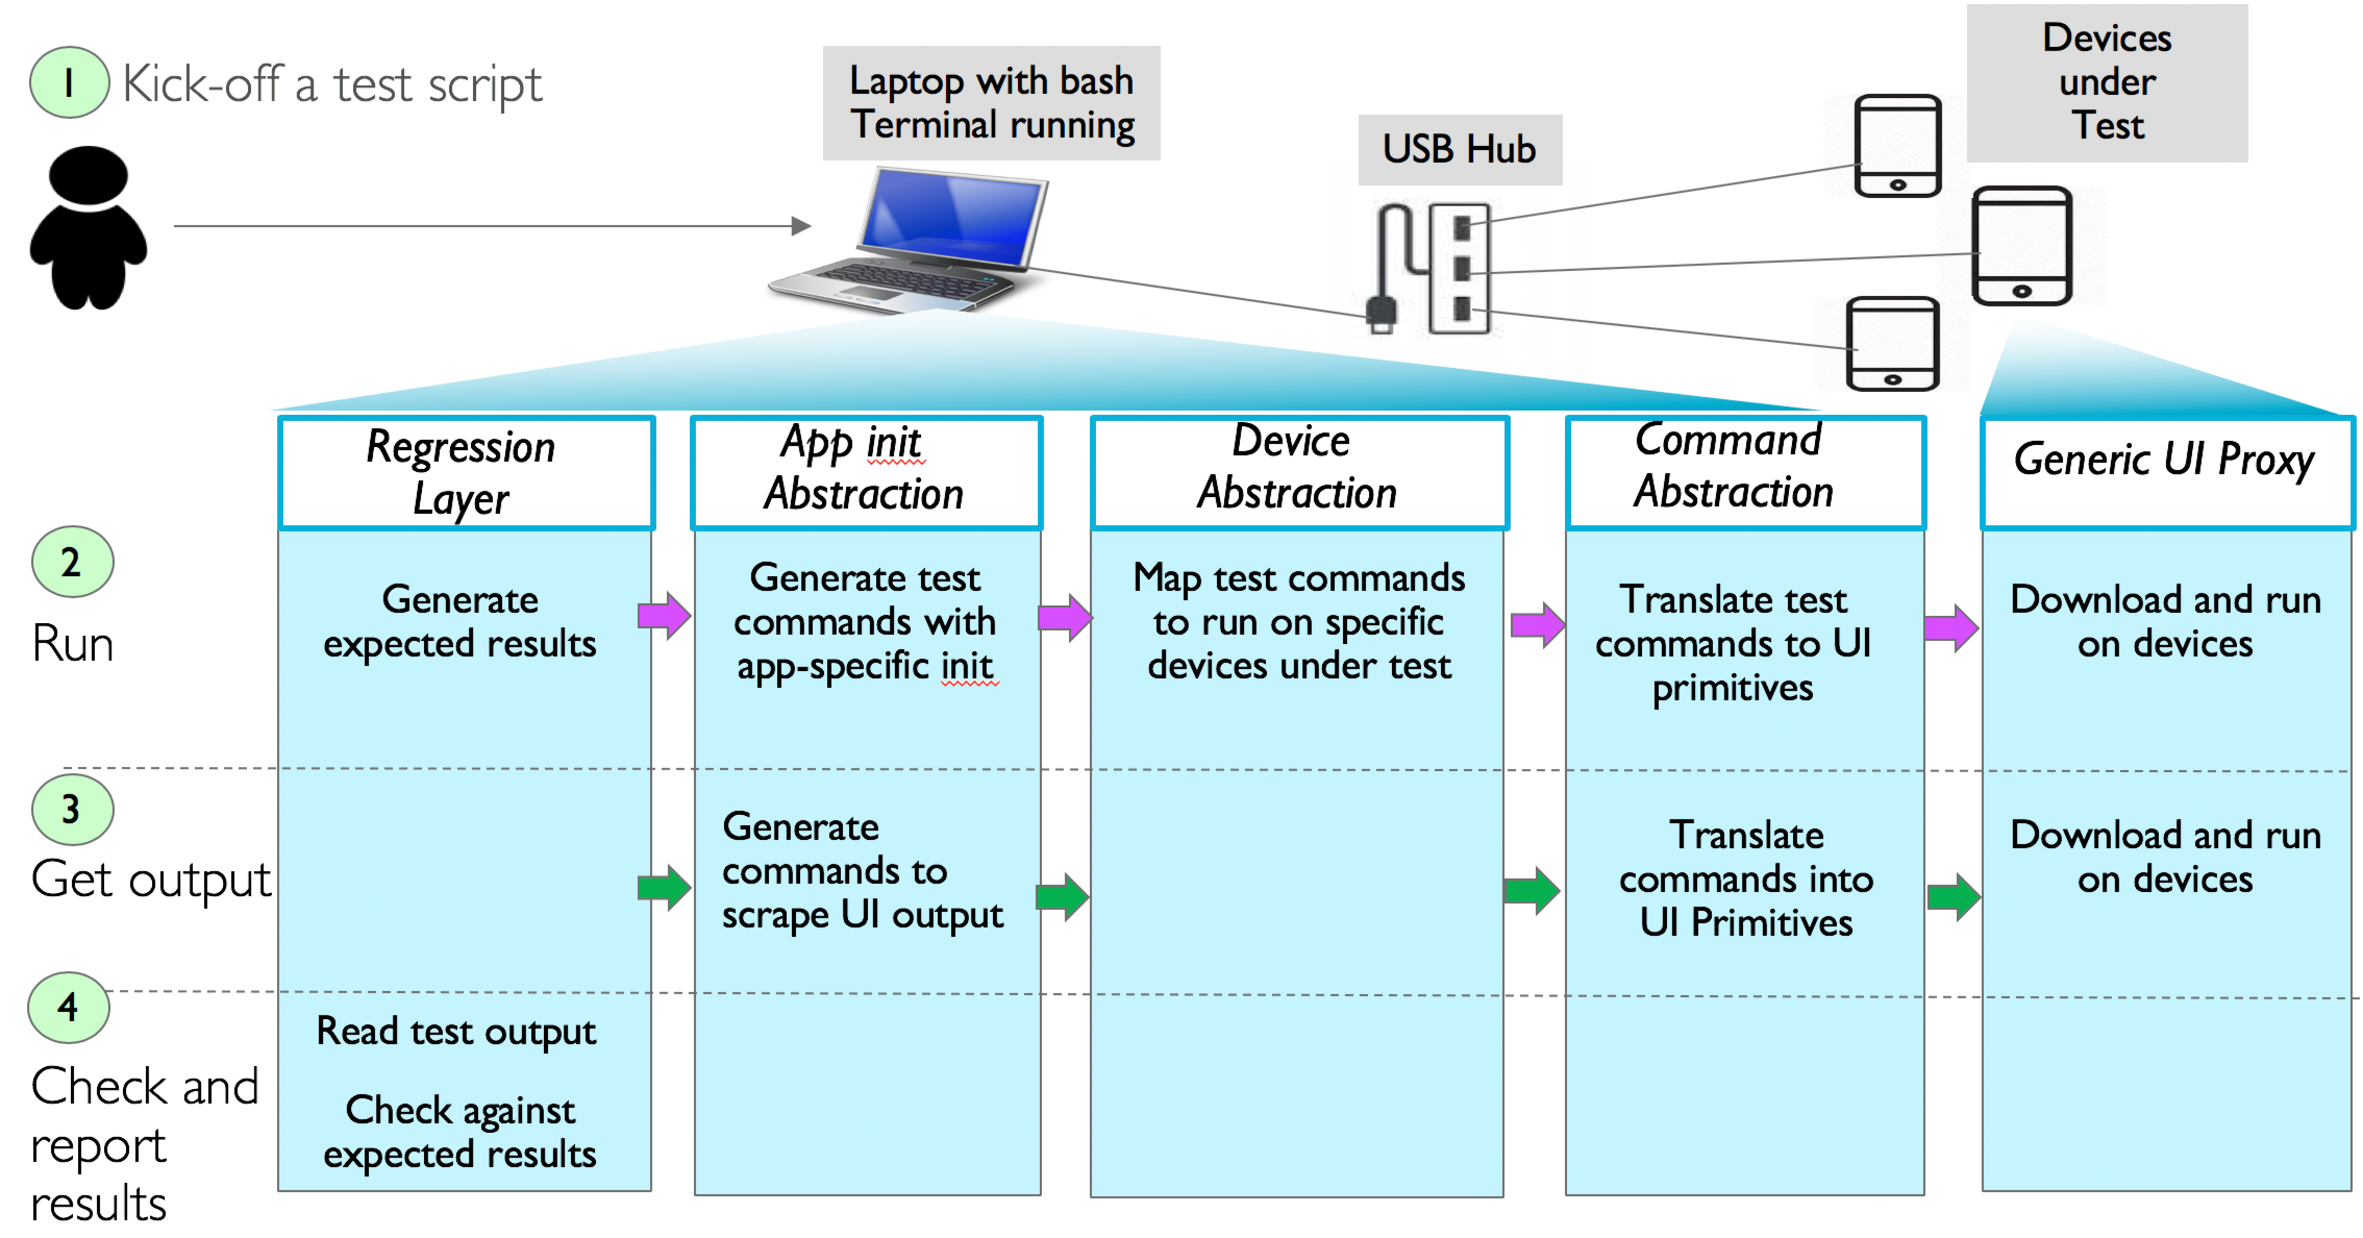
\includegraphics[width=\columnwidth]{figs/test_arch}}
\caption{Automated testing system for MNA}
\label{fig:test_arch}
\end{figure}

We overcame these challenges via innovative techniques, without
resorting to hacks that may violate user security or Appstore
guidelines. With our technique, exchange of information happens
without making network connections. As we describe later, this is
achieved by splitting the messages into small enough chunks so that
they can be stuffed into service advertisements themselves and
broadcast over multiple advertisements in a quick succession.

Our approach here is two-pronged. Firstly, via extensive experiments
on a large number of devices, we fine-tune the algorithms governing
the intervals at which discovery and advertisements occur. In a
nutshell, receiving new information during a period causes MNA to be
more aggressive in discovery and advertisement. Similarly, lack of new
information for a period makes the device less aggressive. Secondly,
we allow ``wake up'' messages to be broadcast in the network ahead of
an anticipated severe weather event. When devices receive such
messages, they schedule themselves to remain aggressive during the
specified window of time. Outside of this window, the device can
afford to have long sleep cycles and conserve power. With these
techniques, our testing shows less than 1\% battery consumption per
hour on most device models.

We developed test automation tools and processes such that multiple
devices can be controlled from a single test station and follow
prescribed steps to generate, send, and receives messages to play out
a test scenario. Finally, the framework allows automated analysis of
the observations to determine the test result. This capability was
instrumental in uncovering bugs at a fast pace to meet the aggressive
timeline and avoid the cost of acquisition. Further, the automation
framework is general and can be expressly applied to test other apps
in this fashion.

In our approach, since the origin of weather information is the
Weather Channel service, digital signatures can be attached to all
weather alerts broadcast from the service. The mobile application is
distributed with the corresponding public key so that digital
signatures from the service can be verified. If a message fails such a
verification, it is discarded and not forwarded any further.
\section{Experimental Results}
\label{sec:eval}

\begin{figure}[htbp]
\centerline{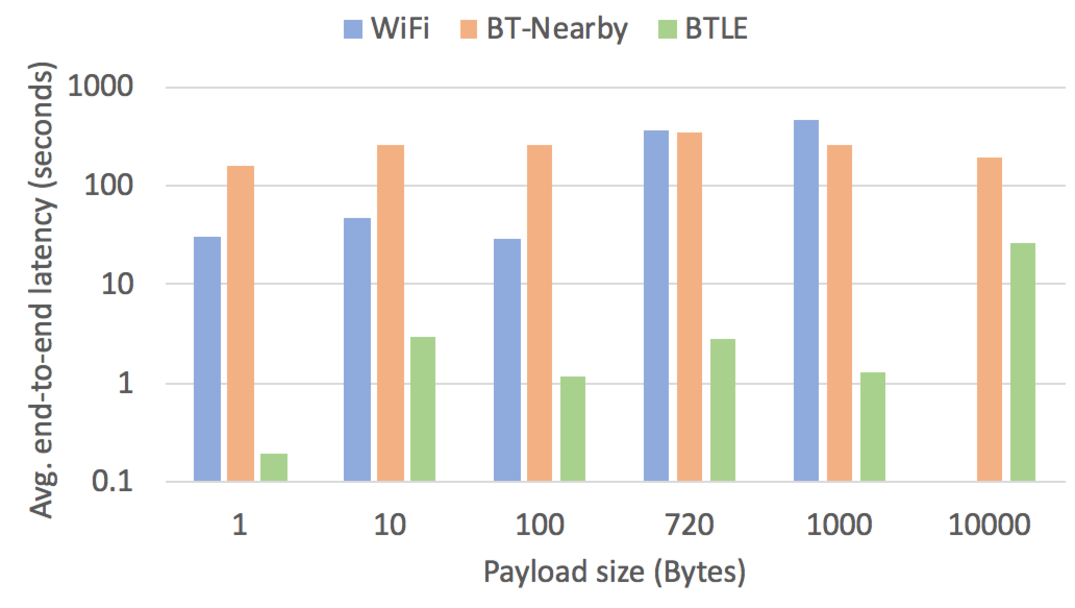
\includegraphics[width=\columnwidth]{figs/e2e_latency}}
\caption{End-to-end latency}
\label{fig:e2e}
\end{figure}

\begin{figure}[htbp]
\centerline{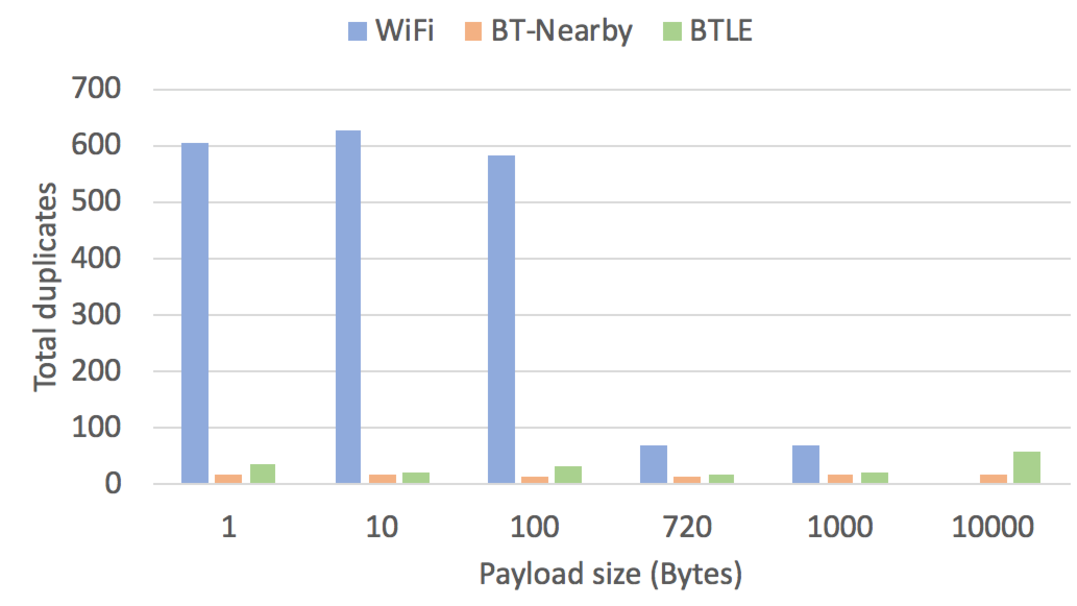
\includegraphics[width=\columnwidth]{figs/duplicates}}
\caption{Duplicity due to flooding}
\label{fig:dup}
\end{figure}

\begin{figure}[htbp]
\centerline{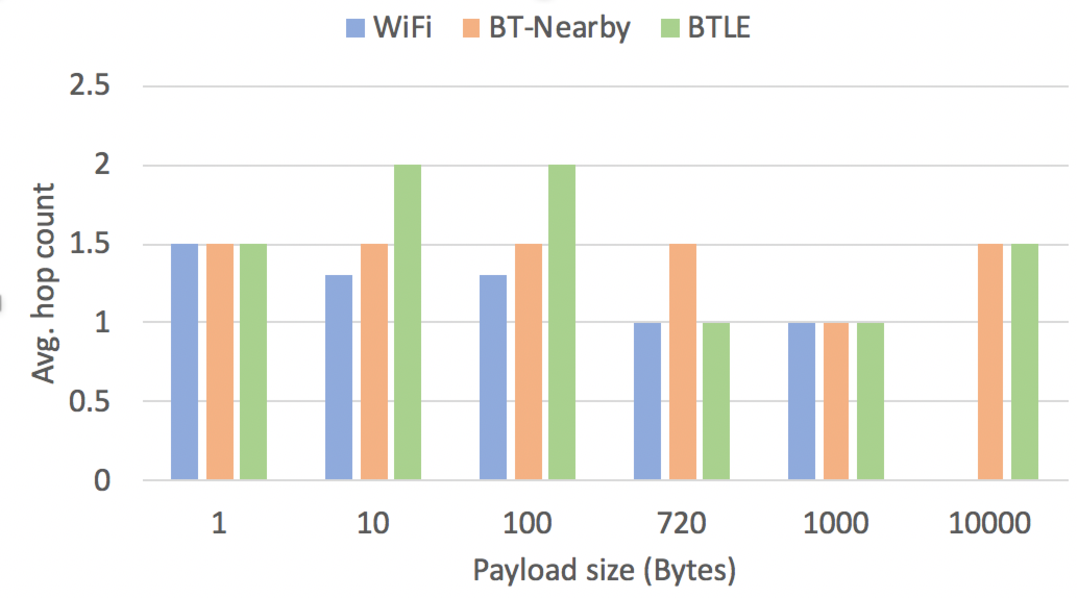
\includegraphics[width=\columnwidth]{figs/hops}}
\caption{Average hop count}
\label{fig:hop}
\end{figure}

%
\section{Related Work}
\label{sec:related}
%
Apart from the state-of-the-art cited earlier, there have been other
notable attempts at practical large-scale deployments and we describe
them here. Before mid-2000’s, most of the research on MANETs was based
on Department of Defense requirements, until commodity multi-hop ad
hoc networks began to be considered \cite{bruno-mesh-2005}. However,
it took another decade before wireless mesh networking was used
commercially to enable smartphones to connect via Bluetooth and WiFi
in a popular application called FireChat \cite{firechat}. The success
of FireChat, partially due to the news coverage of its use in
political situations in which governments restricted access to the
Internet, has led to many alternatives in the past few years. An
up-to-date list of such applications is available
here \footnote{https://alternativeto.net/software/firechat-by-open-garden/}
\section{Conclusions and Future Work}
\label{sec:conclude}

\section*{Acknowledgment}
This research was sponsored by the U.S. Army Research Laboratory and
the U.K. Ministry of Defence under Agree- ment Number
W911NF-16-3-0001. The views and conclusions contained in this document
are those of the authors and should not be interpreted as representing
the official policies, either expressed or implied, of the U.S. Army
Research Laboratory, the U.S. Government, the U.K. Ministry of Defence
or the U.K. Government. The U.S. and U.K. Governments are au- thorized
to reproduce and distribute reprints for Government purposes
notwithstanding any copyright notation hereon.
\bibliographystyle{abbrv} \bibliography{smartcomp19}

\end{document}
